\documentclass{../homework}

\homework{13}
\author{}
\date{Tuesday 5/7}

\begin{document}
\begin{problems}
\item[P.14.27] Let \(T\) be the Volterra operator on \(C[0, 1]\); see
  P.5.11 and P.8.27.
  \begin{book}
    \begin{center}
      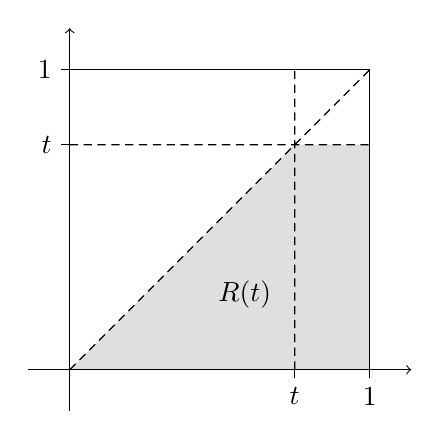
\begin{tikzpicture}[scale=3/2]
        \draw [->] (-1em,0) -- (1in+1em,0);
        \draw [->] (0,-1em) -- (0,1in+1em);

        \fill [opacity=1/8]
        (0,0) -- (1in,0) -- (1in,3in/4) -- (3in/4,3in/4) -- cycle;

        \draw [densely dashed]
        (3in/4,0) -- +(0,1in) node [near start, left=1em/2] {\(R(t)\)}
        (0,3in/4) -- +(1in,0)
        (0,0) -- (1in,1in);

        \draw (0,1in) -| (1in,0);

        \draw
        (0,1in) -- +(-2pt,0) node [left] {\(1\)}
        (0,3in/4) -- +(-2pt,0) node [left] {\(t\)}
        (3in/4,0) -- +(0,-2pt) node [below] {\(t\)}
        (1in,0) -- +(0,-2pt) node [below] {\(1\)};
      \end{tikzpicture}
      \bookfigure{fig:14.3}{14.3}{The region \(R(t)\) in P.14.27.}
    \end{center}
  \end{book}
  \begin{enumerate}
  \item Show that
    \[
      (TT^* f)(t) = \int_0^1 \min(t,s) f(s) \dif s
      \tag{14.4.1}
    \]
    and
    \[
      (T^* Tf)(t) = \int_0^1 \min(1-t, 1-s) f(s) \dif s.
    \]
    \textit{Hint}: Express \((TT^* f)(t)\) as a double integral over
    the region \(R(t)\) in Figure 14.3.

    \begin{solution}
      \begin{proof}

      \end{proof}
    \end{solution}

  \item Deduce that
    \[
      \Inner{T^* f, T^* f} = \int_0^1 \int_0^1
      \min(t, s) f(s) \overline{f(t)} \dif s \dif t \ge 0
      \qquad \text{for all \(f \in C[0, 1]\).}
    \]

    \begin{solution}
      \begin{proof}

      \end{proof}
    \end{solution}

  \item Show that
    \(\Paren{\pi^{-2} \Paren{n + \frac 1 2}^{-2}, \sin\Paren{\pi
        \Paren{n + \frac 1 2} t}}\), \(n = 0, 1, 2, \dots\), are
    eigenpairs of \(T T^*\).  For a discrete analog of (14.4.1), see
    P.13.20.

    \begin{solution}
      \begin{proof}

      \end{proof}
    \end{solution}
  \end{enumerate}

\item[P.15.17] Verify that
  \[
    A^\dagger = \frac{1}{10}
    \begin{bmatrix}
      -2 & -1 & 0 & 1 & 2 \\ 6 & 4 & 2 & 0 & -2
    \end{bmatrix}
  \]
  is the pseudoinverse of the matrix \(A\) in Example 7.5.7 and show
  that \(A^\dagger \vec y\) gives the parameters of the least squares
  line in that example.

  \begin{bookexample}[7.5.7]
    Find a least squares line \(y = ax + b\) to model the data
    \[
      (0,1), (1,1), (2,3), (3,3), (4,4).
    \]
    According to the preceding recipe we have
    \[
      A =
      \begin{bmatrix}
        0 & 1 \\ 1 & 1 \\ 2 & 1 \\ 3 & 1 \\ 4 & 1
      \end{bmatrix},
      \vec x = \begin{bmatrix} a \\ b \end{bmatrix},
      \vec y = \begin{bmatrix} 1 \\ 1 \\ 3 \\ 3 \\ 4 \end{bmatrix},
    \]
    and we solve
    \[
      \underbrace{
        \begin{bmatrix} 30 & 10 \\ 10 & 5 \end{bmatrix}
      }_{A^* A}
      \begin{bmatrix} a \\ b \end{bmatrix}
      = \underbrace{
        \begin{bmatrix} 32 \\ 12 \end{bmatrix}
      }_{A^* \vec y},
    \]
    for \(a = b = \frac 4 5\).  Therefore, the least squares line is
    \(\frac 4 5 x + \frac 4 5\); see Figure 7.10.
  \end{bookexample}

  \begin{solution}
    \begin{proof}

    \end{proof}
  \end{solution}

\item[P.15.23] Let
  \[
    A = \begin{bmatrix} 1 & 0 \\ 0 & 2 \end{bmatrix}
    \qquad\text{and}\qquad
    B = \begin{bmatrix} 1 & 1 \\ 1 & 1 \end{bmatrix}.
  \]
  Show that \((AB)^\dagger \ne B^\dagger A^\dagger\).

  \begin{solution}
    \begin{proof}

    \end{proof}
  \end{solution}

\item[P.15.36] Let \(A \in \M_{m \times n}\).  Show that
  \(\norm A_2 \le 1\) if and only if \(I_n - A^* A\) is positive
  semidefinite.  A matrix that satisfies either of these conditions is
  a \emph{contraction}.

  \begin{solution}
    \begin{proof}

    \end{proof}
  \end{solution}

\item[P.15.39] Let \(C \in \M_n\) be a contraction.  Show that there
  are unitary \(U, V \in \M_n\) such that \(C = \frac 1 2 (U + V)\).
  \textit{Hint}: If \(0 \le \sigma \le 1\) and
  \(s_\pm = \sigma \pm i \sqrt{i-\sigma^2}\), then
  \(\sigma = \frac 1 2 \Paren{s_+ + s_-}\) and \(\Abs{s_\pm} = 1\).

  \begin{solution}
    \begin{proof}

    \end{proof}
  \end{solution}

\item[P.15.40] Deduce from the preceding problem that every square
  matrix is a linear combination of at most two unitary matrices.  See
  P.13.39 for a related result.

  \begin{solution}
    \begin{proof}

    \end{proof}
  \end{solution}

\item[P.15.41] Let \(A, B \in \M_n\) and let \(p\) be a polynomial.
  \begin{enumerate}
  \item Show that \(B p(AB) = p(BA) B\).

    \begin{solution}
      \begin{proof}

      \end{proof}
    \end{solution}

  \item If \(A\) is a contraction, use (a) to show that
    \[
      A^* \Paren{I-AA^*}^{1/2} = \Paren{I-A^* A}^{1/2} A^*.
      \tag{15.9.5}
    \]

    \begin{solution}
      \begin{proof}

      \end{proof}
    \end{solution}
  \end{enumerate}

\item[P.15.43] Let \(A \in \M_n\).  Show that \(A\) is a contraction
  if and only if for some \(m \ge n\), there is a block matrix of the
  form
  \[
    U = \begin{bmatrix} A & B \\ C & D \end{bmatrix} \in \M_m
  \]
  that is unitary.  Thus, every contraction is a principal submatrix
  of some unitary matrix.  \textit{Hint}: Start with
  \(B = \Paren{I - AA^*}^{1/2}\).

  \begin{solution}
    \begin{proof}

    \end{proof}
  \end{solution}
\end{problems}
\end{document}